\chapter{Zupełność przestrzeni metrycznych i twierdzenie Baire'a}
\label{ch:topog-baire}

\noindent\textbf{Cel rozdziału.}
Metryzowalność przestrzeni topologicznej oznacza istnienie metryki
zgodnej z jej topologią (rozdział~10). Zupełność zależy natomiast
od konkretnej metryki. Przedstawimy pojęcie ciągu Cauchy'ego,
odróżnimy zupełność od zupełnej metryzowalności i udowodnimy
twierdzenie Baire'a w dwóch podstawowych wersjach:
dla zupełnych przestrzeni metrycznych oraz lokalnie zwartych
przestrzeni Hausdorffa. Zastosowania dotyczą kategorii Baire'a.

\section{Ciągi Cauchy'ego i zupełność}
\label{sec:topog-baire-zupelnosc}

\begin{definicja}[Ciąg Cauchy'ego i przestrzeń zupełna]
\label{def:topog-baire-ciag-cauchyego}
Niech $(X,d)$ będzie przestrzenią metryczną.
Ciąg $(x_n)_{n\ge1}$ w $X$ jest \emph{ciągiem Cauchy'ego},
jeżeli dla każdego $\varepsilon>0$ istnieje $N\ge1$ takie,
że $d(x_m,x_n)<\varepsilon$ dla wszystkich $m,n\ge N$.
Przestrzeń $(X,d)$ jest \emph{zupełna}, jeżeli każdy
jej ciąg Cauchy'ego jest zbieżny w $X$.
\end{definicja}

\begin{stwierdzenie}[Ciąg zbieżny jest ciągiem Cauchy'ego]
\label{prop:topog-baire-zbiezny-cauchy}
W każdej przestrzeni metrycznej $(X,d)$ ciąg zbieżny
jest ciągiem Cauchy'ego i ma dokładnie jedną granicę.
\end{stwierdzenie}
\begin{proof}
Jeżeli $x_n\to x$, to dla $\varepsilon>0$ dobieramy $N$
z $d(x_n,x)<\varepsilon/2$ dla $n\ge N$.
Dla $m,n\ge N$ nierówność trójkąta daje
$d(x_m,x_n)\le d(x_m,x)+d(x,x_n)<\varepsilon$.
Jeśli jednocześnie $x_n\to y$, to
$d(x,y)\le d(x,x_n)+d(x_n,y)\to0$, skąd $x=y$.
\end{proof}

\begin{twierdzenie}[Zupełność podprzestrzeni]
\label{thm:topog-baire-podprzestrzen-zupelna}
Niech $(X,d)$ będzie zupełną przestrzenią metryczną
i $A\subseteq X$. Przestrzeń $(A,d|_{A\times A})$
jest zupełna wtedy i tylko wtedy, gdy $A$ jest domknięty w $X$.
\end{twierdzenie}
\begin{proof}
Jeśli $A$ jest domknięty, każdy ciąg Cauchy'ego
$(a_n)$ w $A$ jest też ciągiem Cauchy'ego w $X$.
Zbiega zatem do $x\in X$, a ponieważ $a_n\in A$,
mamy $x\in\overline A=A$.

Odwrotnie, załóżmy, że $A$ jest zupełna, i weźmy
$x\in\overline A$. Dla każdego $n$ znajdziemy
$a_n\in A$ z $d(a_n,x)<1/n$. Wtedy $a_n\to x$,
więc $(a_n)$ jest ciągiem Cauchy'ego w $A$.
Z zupełności otrzymujemy $a_n\to a$ dla pewnego
$a\in A$. Jednoznaczność granicy w $X$ daje
$x=a\in A$, zatem $A$ jest domknięty.
\end{proof}

\begin{przyklad}[Przestrzenie zupełne i niezupełne]
\label{ex:topog-baire-podstawowe-przyklady}
Prosta $(\R,|\cdot|)$ jest zupełna. Rzeczywiście,
każdy ciąg Cauchy'ego w $\R$ jest ograniczony
(od pewnego miejsca jego wyrazy są w odległości
mniejszej niż $1$ od ustalonego wyrazu).
Na mocy twierdzenia Bolzana--Weierstrassa
ma więc podciąg zbieżny. Jeśli $x_{n_k}\to x$,
to dla dowolnego $\varepsilon>0$ wybieramy $N$
z $|x_m-x_n|<\varepsilon/2$ dla $m,n\ge N$,
a następnie $k$ z $n_k\ge N$ i
$|x_{n_k}-x|<\varepsilon/2$. Dla $n\ge N$
otrzymujemy $|x_n-x|<\varepsilon$, czyli
zbiega cały ciąg.

Przedział $[0,1]$ jest zupełny jako domknięty
podzbiór $\R$. Przedział $(0,1)$ ze zwykłą
metryką nie jest zupełny, gdyż $1/(n+1)$
jest ciągiem Cauchy'ego bez granicy w $(0,1)$.
Podobnie $\Q$ z metryką odziedziczoną z $\R$
nie jest zupełna: wymierne przybliżenia liczby
$\sqrt2$ tworzą ciąg Cauchy'ego bez granicy w $\Q$.
\end{przyklad}

\begin{definicja}[Zupełna metryzowalność]
\label{def:topog-baire-zupelna-metryzowalnosc}
Przestrzeń topologiczna $X$ jest
\emph{zupełnie metryzowalna}, jeżeli istnieje
co najmniej jedna metryka zupełna na $X$
zgodna z jego topologią.
\end{definicja}

\begin{przyklad}[Zupełność metryki nie jest własnością topologiczną]
\label{ex:topog-baire-metryka-przedzial}
Homeomorfizm $h\colon(0,1)\to\R$,
$h(t)=\tan(\pi(t-\tfrac12))$, przenosi na $(0,1)$
metrykę $d_h(s,t)=|h(s)-h(t)|$. Z rozdziału~10
wiemy, że jest ona zgodna ze zwykłą topologią.
Jest zupełna, bo $h$ jest izometrią na zupełną
przestrzeń $(\R,|\cdot|)$. Tymczasem zwykła
metryka $|s-t|$ na $(0,1)$ nie jest zupełna.
A zatem zupełność metryki nie jest niezmiennikiem
topologicznym. Natomiast zupełna metryzowalność
jest niezmiennikiem topologicznym: jeśli
$g\colon X\to Y$ jest homeomorfizmem, a $e$ jest
zgodną metryką zupełną na $Y$, to metryka
$e_g(x,x')=e(g(x),g(x'))$ jest zgodna z topologią
$X$ (rozdział~10), a $g$ jest izometrią
$(X,e_g)$ na $(Y,e)$, więc $(X,e_g)$ jest zupełna.
\end{przyklad}

\section{Nigdziegęstość i kategorie zbiorów}
\label{sec:topog-baire-kategorie}

\begin{definicja}[Pierwsza kategoria, rezydualność, przestrzeń Baire'a]
\label{def:topog-baire-kategoria}
Niech $X$ będzie przestrzenią topologiczną.
Zbiór $A\subseteq X$ jest \emph{nigdziegęsty},
jeżeli $\operatorname{int}_X(\overline A^{\,X})
=\varnothing$. Zbiór $M\subseteq X$ jest
\emph{pierwszej kategorii} (albo \emph{mizerny}),
jeśli istnieją nigdziegęste zbiory $A_n\subseteq X$,
$n\ge1$, takie, że $M\subseteq\bigcup_{n\ge1}A_n$.
Zbiór $R\subseteq X$ jest \emph{rezydualny},
jeśli $X\setminus R$ jest pierwszej kategorii.
Przestrzeń $X$ jest \emph{przestrzenią Baire'a},
jeżeli każde przeliczalne przecięcie
zbiorów otwartych i gęstych w $X$ jest gęste w $X$.
\end{definicja}

\begin{uwaga}[Kategoria i miara]
Zbiór pierwszej kategorii może być gęsty,
a nigdziegęsty nie musi być przeliczalny.
Własność pierwszej kategorii nie oznacza
zerowej miary; kategoria i miara są
odrębnymi sposobami badania wielkości zbioru.
\end{uwaga}

\begin{stwierdzenie}[Równoważne warunki Baire'a]
\label{prop:topog-baire-rownowaznosci}
Dla każdej przestrzeni topologicznej $X$
równoważne są:
\begin{enumerate}[label=(\roman*)]
\item $X$ jest przestrzenią Baire'a;
\item każdy zbiór pierwszej kategorii w $X$
ma puste wnętrze w $X$;
\item żaden niepusty zbiór otwarty w $X$
nie jest pierwszej kategorii w $X$.
\end{enumerate}
\end{stwierdzenie}
\begin{proof}
Jeśli $A_n$ są nigdziegęste, to
$G_n=X\setminus\overline{A_n}^{\,X}$
są otwarte i gęste. Z (i) wynika, że
$\bigcap_nG_n$ jest gęste, więc jego
dopełnienie $\bigcup_n\overline{A_n}^{\,X}$
ma puste wnętrze. Każdy zbiór pierwszej
kategorii zawiera się w takiej sumie:
otrzymujemy (ii). Implikacja (ii)$\Rightarrow$(iii)
jest natychmiastowa.

Załóżmy (iii). Dla dowolnych zbiorów
otwartych i gęstych $G_n$ dopełnienia
$F_n=X\setminus G_n$ są nigdziegęste.
Gdyby $\bigcap_nG_n$ nie było gęste,
istniałby niepusty zbiór otwarty
$U\subseteq X\setminus\bigcap_nG_n
=\bigcup_nF_n$. Oznaczałoby to, że
$U$ jest pierwszej kategorii w $X$,
wbrew (iii).
\end{proof}

\section{Twierdzenie Baire'a w przestrzeniach zupełnych}
\label{sec:topog-baire-twierdzenie-metryczne}

\begin{twierdzenie}[Twierdzenie Baire'a o kategorii --- wersja metryczna]
\label{thm:topog-baire-metryczne}
Jeśli $(X,d)$ jest zupełną przestrzenią metryczną,
a $(G_n)_{n\ge1}$ jest ciągiem zbiorów otwartych
i gęstych w $X$, to dla każdego niepustego
otwartego $U\subseteq X$ zachodzi
$U\cap\bigcap_{n\ge1}G_n\ne\varnothing$.
W szczególności $X$ jest przestrzenią Baire'a.
\end{twierdzenie}
\begin{proof}
Zbiór $U\cap G_1$ jest niepusty i otwarty.
Wybierzmy $x_1\in U\cap G_1$ oraz
$r_1\in(0,2^{-1})$ tak mały, że
$K_1=\{y\in X:d(x_1,y)\le r_1\}
\subseteq U\cap G_1$.

Załóżmy, że mamy już niepustą domkniętą kulę
$K_n=\{y:d(x_n,y)\le r_n\}$, gdzie
$0<r_n<2^{-n}$. Gęstość $G_{n+1}$
zapewnia istnienie punktu
$x_{n+1}\in B_d(x_n,r_n)\cap G_{n+1}$.
Z otwartości tego przecięcia możemy
wybrać $0<r_{n+1}<2^{-(n+1)}$ tak, aby
\[
K_{n+1}:=\{y:d(x_{n+1},y)\le r_{n+1}\}
\subseteq B_d(x_n,r_n)\cap G_{n+1}.
\]
Stąd $K_1\supseteq K_2\supseteq\cdots$
oraz $K_n\subseteq G_n$ dla wszystkich $n$.

Dla $m>n$ mamy $x_m\in K_n$, skąd
$d(x_m,x_n)\le r_n<2^{-n}$. Ciąg $(x_n)$
jest zatem ciągiem Cauchy'ego i na mocy
zupełności zbiega do pewnego $x\in X$.
Przy ustalonym $n$ wszystkie $x_m$ dla
$m\ge n$ należą do domkniętego $K_n$,
więc również granica $x$ należy do $K_n$.
Otrzymujemy
$x\in\bigcap_nK_n\subseteq
U\cap\bigcap_nG_n$, co kończy dowód.
\end{proof}

\begin{figure}[htbp]
\centering
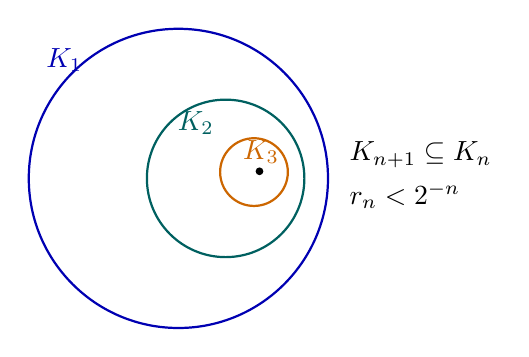
\begin{tikzpicture}
\draw[blue!70!black,thick] (0,0) circle (1.9);
\draw[teal!75!black,thick] (.6,0) circle (1.0);
\draw[orange!80!black,thick] (.96,.08) circle (.43);
\fill (1.03,.09) circle (1.4pt);
\node[blue!70!black] at (-1.45,1.5) {$K_1$};
\node[teal!75!black] at (.22,.7) {$K_2$};
\node[orange!80!black] at (1.05,.33) {$K_3$};
\node[anchor=west] at (2.05,.3) {$K_{n+1}\subseteq K_n$};
\node[anchor=west] at (2.05,-.22) {$r_n<2^{-n}$};
\end{tikzpicture}
\caption{Schemat konstrukcji zstępujących kul domkniętych.
Rysunek ilustruje inkluzje, a nie rzeczywiste zanurzenie
dowolnej przestrzeni metrycznej w płaszczyźnie.}
\label{fig:topog-baire-kule}
\end{figure}

\begin{wniosek}[Zupełna metryzowalność a własność Baire'a]
\label{cor:topog-baire-zupelnie-metryzowalne}
Każda przestrzeń zupełnie metryzowalna
jest przestrzenią Baire'a.
\end{wniosek}
\begin{proof}
Wybieramy zgodną metrykę zupełną i stosujemy
twierdzenie~\ref{thm:topog-baire-metryczne}.
Otwartość i gęstość zależą tylko od topologii.
\end{proof}

\section{Twierdzenie Baire'a w przestrzeniach lokalnie zwartych}
\label{sec:topog-baire-lokalnie-zwarte}

\begin{definicja}[Zwartość lokalna]
\label{def:topog-baire-lokalna-zwartosc}
Przestrzeń topologiczna $X$ jest
\emph{lokalnie zwarta}, jeżeli każdy
$x\in X$ ma zwarte otoczenie:
istnieje zwarty $K\subseteq X$
taki, że $x\in\operatorname{int}_X K$.
\end{definicja}

\begin{lemat}[Otoczenia o zwartym domknięciu]
\label{lem:topog-baire-zwarte-domkniecie}
Niech $X$ będzie lokalnie zwartą przestrzenią Hausdorffa.
Dla każdego $x\in X$ i każdego otwartego otoczenia
$V$ punktu $x$ istnieje otwarty $W\ni x$
o zwartym domknięciu $\overline W^{\,X}\subseteq V$.
\end{lemat}
\begin{proof}
Z lokalnej zwartości wybieramy zwarty
$K\subseteq X$ z $x\in\operatorname{int}_X K$.
Przestrzeń $K$ jest zwarta i Hausdorffa,
więc normalna (rozdział~07). Zbiór
$O=V\cap\operatorname{int}_X K$ jest
otwartym otoczeniem $x$ w $K$.
Kryterium zwężania otoczeń w przestrzeni
regularnej (rozdział~05) daje zbiór $H$
otwarty w $K$ spełniający
$x\in H\subseteq\overline H^{\,K}\subseteq O$.
Ponieważ $H\subseteq\operatorname{int}_X K$,
jest on także otwarty w $X$: jeśli
$H=T\cap K$ dla otwartego $T\subseteq X$,
to $H=T\cap\operatorname{int}_X K$.
Przyjmujemy $W=H$. Zwartość $K$
i własność Hausdorffa zapewniają domkniętość
$K$ w $X$ (rozdział~07), toteż
$\overline W^{\,X}=\overline H^{\,K}\subseteq V$.
Domknięty podzbiór zwartego $K$
jest zwarty, co kończy dowód.
\end{proof}

\begin{twierdzenie}[Twierdzenie Baire'a --- wersja lokalnie zwarta]
\label{thm:topog-baire-lokalnie-zwarte}
Każda lokalnie zwarta przestrzeń Hausdorffa
jest przestrzenią Baire'a.
\end{twierdzenie}
\begin{proof}
Niech $U$ będzie niepustym zbiorem otwartym,
a $G_n$ --- otwartymi zbiorami gęstymi.
Wybieramy $x_1\in U\cap G_1$.
Lemat~\ref{lem:topog-baire-zwarte-domkniecie}
daje niepusty otwarty $W_1$ o niepustym
zwartym domknięciu $K_1\subseteq U\cap G_1$.

Indukcyjnie, mając niepusty otwarty $W_n$
o zwartym domknięciu $K_n$, wybieramy
$x_{n+1}\in W_n\cap G_{n+1}$
i na mocy lematu otrzymujemy niepusty otwarty
$W_{n+1}$, którego zwarte domknięcie
$K_{n+1}$ zawiera się w $W_n\cap G_{n+1}$.
Zbiory $K_n$ są więc niepuste, zstępujące,
domknięte w $X$ (gdyż $X$ jest Hausdorffa)
i wszystkie zawierają się w zwartym $K_1$.

Gdyby $\bigcap_{n\ge1}K_n=\varnothing$,
to otwarte w $K_1$ zbiory $K_1\setminus K_n$
tworzyłyby pokrycie $K_1$. Ze zwartości
istniałoby podpokrycie skończone,
a ponieważ $(K_n)$ jest zstępujący,
oznaczałoby to $K_N=\varnothing$ dla
pewnego $N$. Jest to sprzeczność.
Zatem $\bigcap_nK_n$ jest niepuste
i zawiera się w $U\cap\bigcap_nG_n$.
\end{proof}

\section{Konsekwencje i kontrprzykłady}
\label{sec:topog-baire-przyklady}

\begin{przyklad}[Zbiór wymiernych jest mizerny i gęsty]
\label{ex:topog-baire-wymierne}
Każdy singleton $\{q\}$ jest nigdziegęsty
w $\R$, ponieważ jest domknięty i ma puste wnętrze.
Ponieważ $\Q$ jest przeliczalny, jest pierwszej
kategorii w $\R$, choć jednocześnie jest gęsty.
Natomiast $\R\setminus\Q$ jest rezydualny
i gęsty w $\R$.
\end{przyklad}

\begin{twierdzenie}[Zbiór wymiernych nie jest zbiorem $G_\delta$]
\label{thm:topog-baire-wymierne-nie-gdelta}
Zbioru $\Q$ nie można przedstawić jako
przeliczalnego przecięcia zbiorów otwartych w $\R$.
\end{twierdzenie}
\begin{proof}
Załóżmy, że $\Q=\bigcap_{n\ge1}U_n$,
gdzie $U_n$ są otwarte w $\R$.
Ponieważ $\Q$ jest gęsty, wszystkie $U_n$
są gęste. Wypiszmy $\Q=\{q_n:n\ge1\}$.
Każdy $V_n=\R\setminus\{q_n\}$ jest
otwarty i gęsty. Z twierdzenia Baire'a
dla zupełnej prostej $\R$ wynika,
że przecięcie $\bigcap_n(U_n\cap V_n)$
jest gęste i w szczególności niepuste.
Tymczasem jest równe
$\Q\cap(\R\setminus\Q)=\varnothing$.
Sprzeczność.
\end{proof}

\begin{przyklad}[Metryzowalność nie wystarcza]
\label{ex:topog-baire-q-nie-baire}
Przestrzeń $\Q$ z topologią odziedziczoną
z $\R$ jest metryzowalna, ale nie jest Baire'a.
Dla każdego $q\in\Q$ singleton $\{q\}$
jest domknięty i ma puste wnętrze w $\Q$,
więc $\Q$ jest pierwszej kategorii w sobie.
Jest zarazem niepustym otwartym zbiorem
w sobie, co przeczy
stwierdzeniu~\ref{prop:topog-baire-rownowaznosci}(iii).
\end{przyklad}

\begin{stwierdzenie}[Otwarte podprzestrzenie przestrzeni Baire'a]
\label{prop:topog-baire-otwarte-podprzestrzenie}
Jeżeli $X$ jest przestrzenią Baire'a,
a $U\subseteq X$ jest otwarty,
to $U$ z topologią podprzestrzeni
jest przestrzenią Baire'a.
\end{stwierdzenie}
\begin{proof}
Niech $V\subseteq U$ będzie niepusty i otwarty
w $U$, a $H_n\subseteq U$ będą otwarte i gęste w $U$.
Ponieważ $U$ jest otwarty w $X$, także $V$
i $H_n$ są otwarte w $X$. Definiujemy
$G_n=H_n\cup(X\setminus\overline U^{\,X})$.
Zbiory $G_n$ są otwarte w $X$.
Ponieważ $H_n$ jest gęsty w $U$,
jego domknięcie w $X$ zawiera $\overline U^{\,X}$.
Wobec tego $G_n$ jest gęsty w $X$.
Własność Baire'a przestrzeni $X$ daje
$x\in V\cap\bigcap_nG_n$.
Ponieważ $V\subseteq U$ i $G_n\cap U=H_n$,
mamy $x\in V\cap\bigcap_nH_n$.
\end{proof}

\begin{uwaga}[Własność Baire'a a zupełność]
Przedział $(0,1)$ z metryką euklidesową
nie jest zupełny, ale jest przestrzenią Baire'a
jako otwarta podprzestrzeń $\R$.
Jest on również zupełnie metryzowalny
na mocy przykładu~\ref{ex:topog-baire-metryka-przedzial}.
Wersja metryczna twierdzenia Baire'a
jest więc implikacją, a nie charakteryzacją
zupełności wybranej metryki.
\end{uwaga}

\begin{wniosek}[Przeliczalna suma zbiorów domkniętych]
\label{cor:topog-baire-domkniete}
Niech $X$ będzie niepustą przestrzenią Baire'a.
Jeżeli $X=\bigcup_{n\ge1}F_n$ dla domkniętych
$F_n\subseteq X$, to co najmniej jeden
z $F_n$ ma niepuste wnętrze w $X$.
\end{wniosek}
\begin{proof}
Gdyby każde $F_n$ miało puste wnętrze,
wszystkie byłyby nigdziegęste,
a $X$ byłaby pierwszej kategorii w sobie.
Przeczyłoby to
stwierdzeniu~\ref{prop:topog-baire-rownowaznosci}(iii)
dla niepustego otwartego zbioru $X$.
\end{proof}

\begin{uwaga}[Związek z analizą funkcjonalną]
Ostatni wniosek to podstawowy argument
w twierdzeniach Banacha--Steinhausa,
o odwzorowaniu otwartym oraz o wykresie domkniętym.
Ich pełne dowody znajdują się w skrypcie
\emph{Analiza funkcjonalna}.
\end{uwaga}
